%%%%%%%%%%%%%%%%%%%%%%%%%%%%%%%%%%%%%%%%%
% Beamer Presentation
% LaTeX Template
% Version 1.0 (10/11/12)
%
% This template has been downloaded from:
% http://www.LaTeXTemplates.com
%
% License:
% CC BY-NC-SA 3.0 (http://creativecommons.org/licenses/by-nc-sa/3.0/)
%
%%%%%%%%%%%%%%%%%%%%%%%%%%%%%%%%%%%%%%%%%

%----------------------------------------------------------------------------------------
%	PACKAGES AND THEMES
%----------------------------------------------------------------------------------------

\documentclass{beamer}

\mode<presentation> {

% The Beamer class comes with a number of default slide themes
% which change the colors and layouts of slides. Below this is a list
% of all the themes, uncomment each in turn to see what they look like.

%\usetheme{default}
%\usetheme{AnnArbor}
%\usetheme{Antibes}
%\usetheme{Bergen}
%\usetheme{Berkeley}
%\usetheme{Berlin}
%\usetheme{Boadilla}
%\usetheme{CambridgeUS}
%\usetheme{Copenhagen}
%\usetheme{Darmstadt}
%\usetheme{Dresden}
%\usetheme{Frankfurt}
%\usetheme{Goettingen}
%\usetheme{Hannover}
%\usetheme{Ilmenau}
%\usetheme{JuanLesPins}
%\usetheme{Luebeck}
\usetheme{Madrid}
%\usetheme{Malmoe}
%\usetheme{Marburg}
%\usetheme{Montpellier}
%\usetheme{PaloAlto}
%\usetheme{Pittsburgh}
%\usetheme{Rochester}
%\usetheme{Singapore}
%\usetheme{Szeged}
%\usetheme{Warsaw}

% As well as themes, the Beamer class has a number of color themes
% for any slide theme. Uncomment each of these in turn to see how it
% changes the colors of your current slide theme.

%\usecolortheme{albatross}
%\usecolortheme{beaver}
%\usecolortheme{beetle}
%\usecolortheme{crane}
%\usecolortheme{dolphin}
%\usecolortheme{dove}
%\usecolortheme{fly}
%\usecolortheme{lily}
%\usecolortheme{orchid}
%\usecolortheme{rose}
%\usecolortheme{seagull}
%\usecolortheme{seahorse}
%\usecolortheme{whale}
%\usecolortheme{wolverine}

%\setbeamertemplate{footline} % To remove the footer line in all slides uncomment this line
%\setbeamertemplate{footline}[page number] % To replace the footer line in all slides with a simple slide count uncomment this line

%\setbeamertemplate{navigation symbols}{} % To remove the navigation symbols from the bottom of all slides uncomment this line
}

\usepackage{graphicx} % Allows including images
\usepackage{booktabs} % Allows the use of \toprule, \midrule and \bottomrule in tables
\usepackage{color, colortbl}
\usepackage{listings}

\lstdefinestyle{code}{basicstyle=\tiny, language=C, tabsize=2, numbers=left, showspaces=false, showstringspaces=false, xleftmargin=5.0ex}

%----------------------------------------------------------------------------------------
%	TITLE PAGE
%----------------------------------------------------------------------------------------

\title[Get-to-know your system]{Get-to-know your system} % The short title appears at the bottom of every slide, the full title is only on the title page

\author{Martin Radev} % Your name
\institute[Microprocessors18] % Your institution as it will appear on the bottom of every slide, may be shorthand to save space
{
\medskip
\textit{} % Your email address
}
\date{\today} % Date, can be changed to a custom date

\begin{document}

\begin{frame}
\titlepage % Print the title page as the first slide
\end{frame}

\begin{frame}
\frametitle{Overview} % Table of contents slide, comment this block out to remove it
\tableofcontents % Throughout your presentation, if you choose to use \section{} and \subsection{} commands, these will automatically be printed on this slide as an overview of your presentation
\end{frame}

%----------------------------------------------------------------------------------------
%	PRESENTATION SLIDES
%----------------------------------------------------------------------------------------

%------------------------------------------------
\section{First Section} % Sections can be created in order to organize your presentation into discrete blocks, all sections and subsections are automatically printed in the table of contents as an overview of the talk
%------------------------------------------------


\begin{frame}
\frametitle{Motivation}
\begin{itemize}
\item Vendors typically don't share all of the info for a chip
\item At a chip company you might implement similar internal verification tests
\item Hands-on experience with how the system works
\end{itemize}
\end{frame}
%------------------------------------------------

\begin{frame}
\frametitle{Determining cache line size}
\begin{itemize}
\item Determine the amortized cost of reading a byte with a given stride
\item Small stride $\rightarrow$ Cache line reuse $\rightarrow$ Small amortized cost
\item Big stride $\rightarrow$ New cache line per read $\rightarrow$ cost of reading a line
\end{itemize}
\end{frame}

\begin{frame}[fragile]
\frametitle{Determining cache line size}
\begin{block}{Code}
\begin{lstlisting}[style=code]
for (u32 stride = 1; stride < 128; ++stride)
{
    u8 tmp;
    u64 va = (u64)buffer;
    u64 t1 = time_start();
    for (c = 0; c < buffer_size; c += stride, va += stride)
    {
        asm volatile(".intel_syntax noprefix\n\t"
                     "mov %0, BYTE [%1]\n\t"
                     ".att_syntax prefix\n\t"
                     : "=r"(tmp)
                     : "r"(va));
    }
    u64 t2 = time_end();
    u64 cyclesPerByte = (t2-t1) / (buffer_size / stride);
}
\end{lstlisting}
\end{block}
\end{frame}

\begin{frame}
\frametitle{Cache line plot}
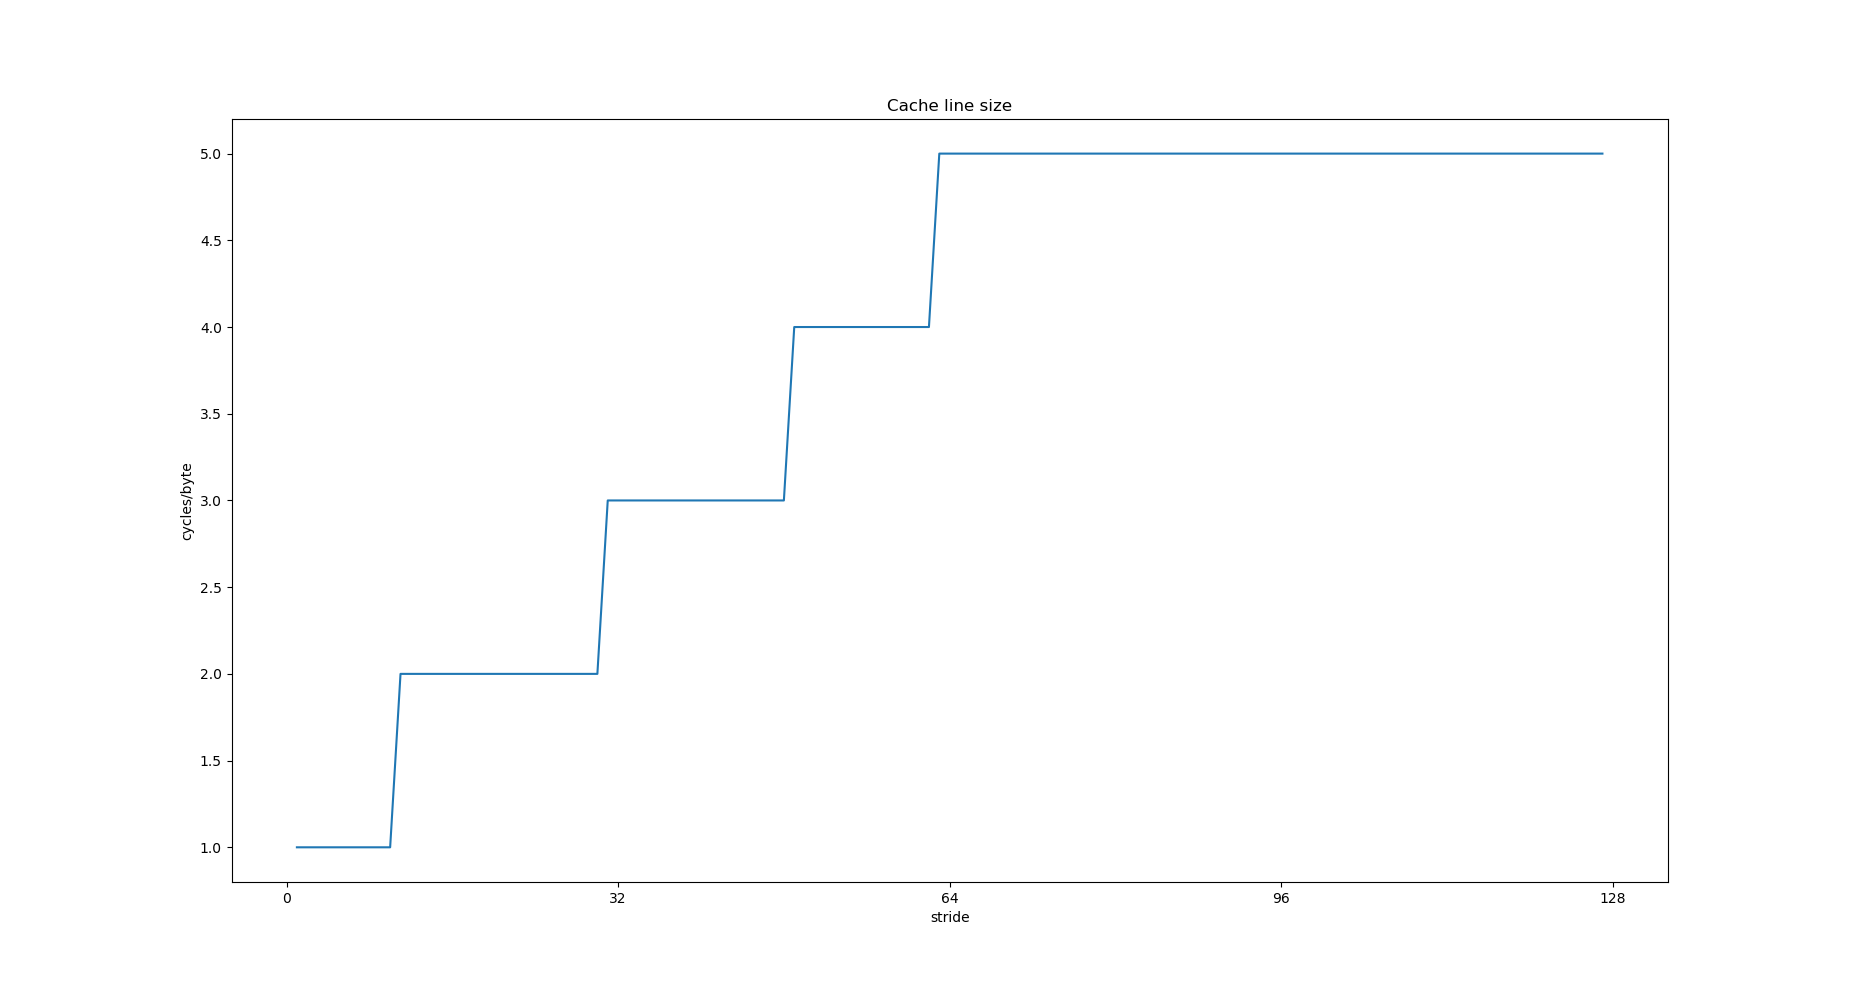
\includegraphics[scale=.24]{img/cache_line_size.png}
\end{frame}

\begin{frame}
\frametitle{Determining data cache size - idea}
\begin{itemize}
\item Vary size of the working set to exercise capacity misses
\item Very small set $\rightarrow$ L1 data cache $\rightarrow$ kind of fast
\item Small set $\rightarrow$ L2 data cache $\rightarrow$ slowish
\item Medium set $\rightarrow$ L3 data cache $\rightarrow$ slow
\item Big set $\rightarrow$ RAM $\rightarrow$ very slow
\item etc
\end{itemize}
\end{frame}

\begin{frame}
\frametitle{Determining data cache size}
\begin{itemize}
\item Working set - continuous portion of virtual memory\\
      Lessen conflict misses
\item Access randomly and uniformly to avoid prefetching
\item Typically done via \textbf{pointer chasing}
\end{itemize}
\begin{center}
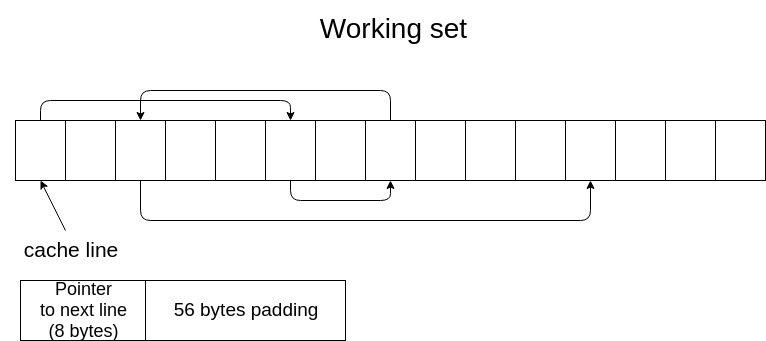
\includegraphics[scale=.3]{img/pchase.jpg}
\end{center}
\end{frame}

\begin{frame}[fragile]
\frametitle{Pointer chasing - sequence generation}
\begin{block}{Code}
\begin{lstlisting}[style=code]
typedef struct BlockDecl
{
    struct BlockDecl *next;
    u8 padding[56U];
} Block;

void generateRandomSequence(Block *blocks, size_t numBlocks)
{
    size_t prevAddr = 0U;
    for (size_t i = 0U; i < numBlocks; ++i)
    {
        size_t nextAddr = (prevAddr + numBlocks - 1U) % numBlocks;
        blocks[prevAddr].next = &blocks[nextAddr];
        prevAddr = nextAddr;
    }
}
\end{lstlisting}
\end{block}
\end{frame}

\begin{frame}[fragile]
\frametitle{Determining data cache size}
\begin{block}{Code}
\begin{lstlisting}[style=code]
const size_t kMaxBlocks = 12*1024U*1024U;
Block *blocks = (Block*)mmap(NULL, sizeof(Block) * kMaxBlocks, PROT_READ|PROT_WRITE,
                             MAP_PRIVATE|MAP_POPULATE|MAP_ANONYMOUS, -1, 0U);
if (blocks == MAP_FAILED)
{
    printf("Failed to allocate: %s\n", strerror(errno));
    return;
}
for (size_t j = 3U; j < kMaxBlocks; j = (j*15U)/11U)
{
    generateRandomSequence(blocks, j);
    size_t kMaxAccesses = kMaxBlocks; // Make sure all blocks are accessed
    size_t numSamples = 4U; 
    u64 t1 = time_start()
    Block *b = &blocks[0]; 
    for (size_t i = 0U; i < kMaxAccesses; ++i)
        b = b->next;
    u64 t2 = time_end();
    PRINT t2-t1
    if (b == NULL) // Prevent compiler from optimizing out the loop above
        exit(1);
}

\end{lstlisting}
\end{block}
\end{frame}

\begin{frame}
\frametitle{Data cache plot - I7 3930K (Sandy bridge)}
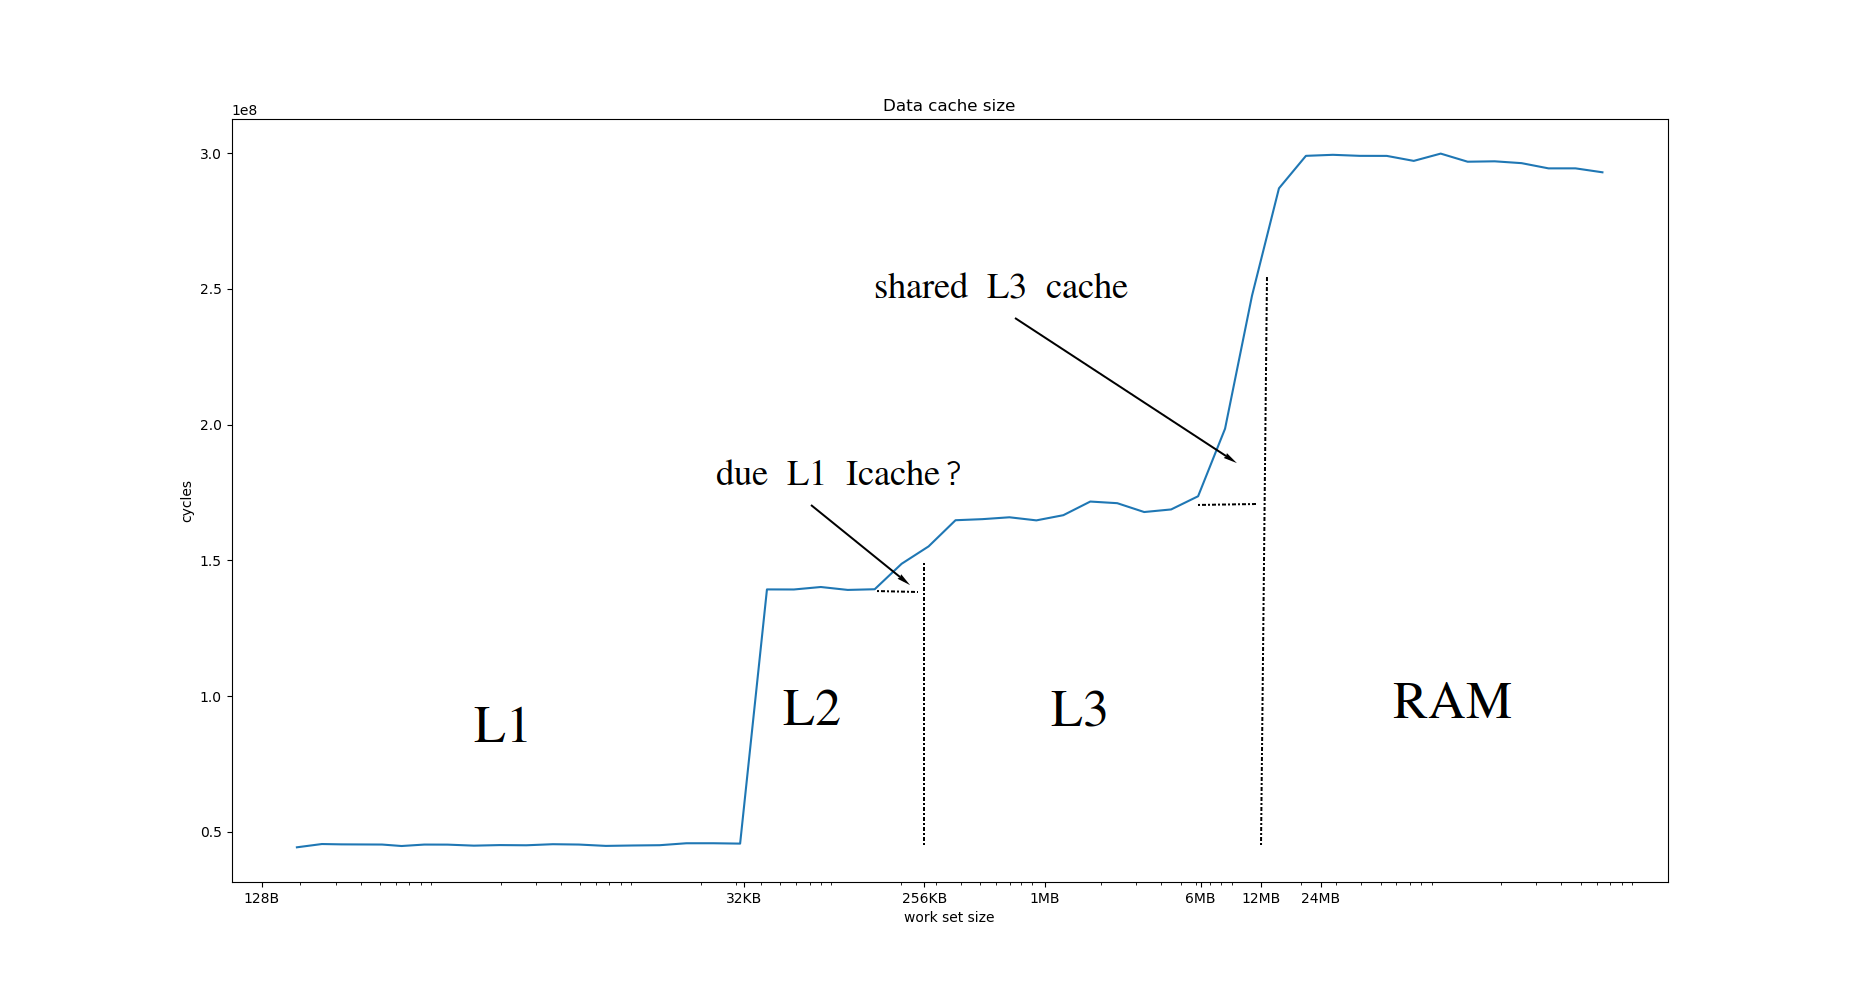
\includegraphics[scale=.18]{img/data_size.png}
\end{frame}

\begin{frame}
\frametitle{Data cache plot - Ryzen 2700X}
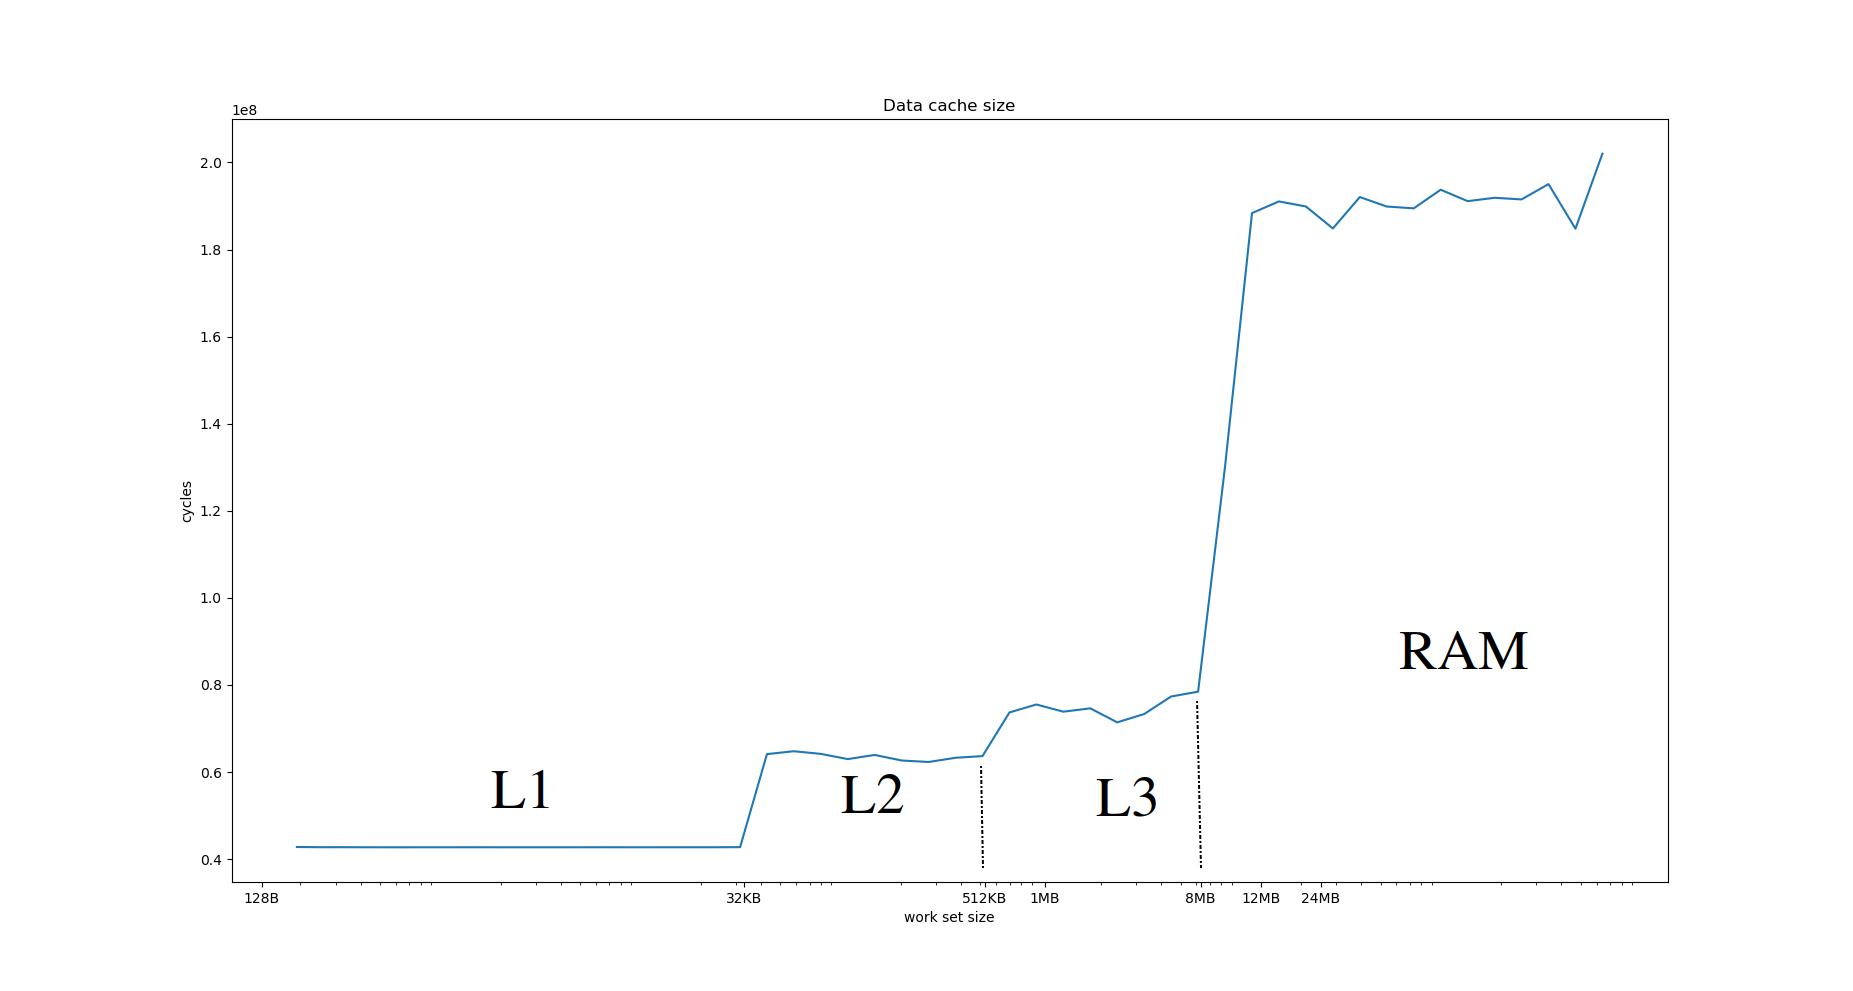
\includegraphics[scale=.25]{img/data_size_zen.png}
\end{frame}

\begin{frame}
\frametitle{What about the instruction cache?}
\begin{itemize}
\item L1 split into I-cache and D-cache 
\item The I-cache could have different parameters
\item Could be determined via pointer chasing again
\item ... But requires some hackery
\end{itemize}
\end{frame}

\begin{frame}[fragile]
\frametitle{Executable virtual pages on Linux}
Three types of pages:\\
\begin{itemize}
\item Readable - R
\item Writable - W
\item Executable - E
\end{itemize}
Data is typically marked as RW for security\\
We can create a mapping tagged with RWE using mmap\\
Thus, we can dynamically generate code and get it to execute :)\\
Other ways out there too - modify the section headers in the exe\\
But your AV SW might complain :)

\begin{block}{Example code}
\begin{lstlisting}[style=code]
mmap(NULL, sizeof(Block) * kMaxBlocks,
     PROT_READ|PROT_WRITE|PROT_EXEC,
     MAP_PRIVATE|MAP_POPULATE|MAP_ANONYMOUS,
     -1, 0U);
\end{lstlisting}
\end{block}
\end{frame}

\begin{frame}[fragile]
\frametitle{Pointer chasing in code}
\begin{itemize}
\item Same idea
\item BUT CPU must fetch instructions from different locations, not data
\item Thus, each cache line has to contain instructions to force the PC (EIP) to change
\end{itemize}
\begin{block}{Example code as it would be in memory}
\begin{lstlisting}[style=code]
u64 t1 = begin_time()
Call function cache_line_1(counter)
u64 t2 = end_time()
print t2-t1
... some other stuff ...

func Cache_line_1(counter)
    decrement counter
    if (counter != 0)
    {
        jump to next random cache line
    }
    return

... some garbage here ...
... many more lines here ...
\end{lstlisting}
\end{block}
\end{frame}

\begin{frame}[fragile]
\frametitle{Translating the code into assembly}
\begin{block}{Pseudo-code}
\begin{lstlisting}[style=code]
func Cache_line_1(counter)
    decrement counter
    if (counter != 0)
    {
        jump to next random cache line
    }
    return
\end{lstlisting}
\end{block}
\begin{block}{The real thing?}
\begin{lstlisting}[style=code]
dec eax ; This modifies the flags
jne 0xBAADA555 ; the address here varies depending on where the next line is located
ret ; in case we don't jump, then return
\end{lstlisting}
\end{block}
Not quite there yet!\\
The CPU doesn't understand mnemonic names\\
It understands machine code
\end{frame}

\begin{frame}[fragile]
\frametitle{Translating assembly into machine code}
The formula:\\
\begin{itemize}
\item Google "dec x86 encoding"
\item Be careful of addressing mode
\item Copy-paste byte values into your C code
\end{itemize}
\begin{block}{The real thing}
FF C8 $\rightarrow$ dec eax\\
0F 85 55 A5 AD BA $\rightarrow$ jne 0xBAADA555\\
C3 $\rightarrow$ ret
\end{block}
\end{frame}

\begin{frame}[fragile]
\frametitle{Measuring L1 I-cache size}
\begin{block}{Code}
\begin{lstlisting}[style=code]
for (size_t j = 64U; j < kMaxBlocks; j += 64) {
    size_t prevAddr = 0U;
    for (size_t i = 0; i < j; ++i) {
        size_t nextAddr = (prevAddr + j - 1U) % j;
        u64 nextBlockVA = (u64)(&blocks[nextAddr]);
        u8 *block = (u8*)&blocks[prevAddr];
        // Determine relative offset to next block
        u64 offset = nextBlockVA - (u64)block;
        u32 offsetU32 = (u32)(offset & 0xFFFFFFFFU);
        u32 offsetU32Adj = offsetU32 - 8U; // 8 bytes since dec and jne take 8 bytes
        block[0] = 0xFFU; block[1] = 0xC8U; // dec eax
        block[2] = 0x0FU; block[3] = 0x85U; // jne
        memcpy(&block[4], &offsetU32Adj, 4U); // relative offset
        block[8] = 0xC3U; // ret
        prevAddr = nextAddr;
    }
    u64 t1 = time_start();
    asm volatile(".intel_syntax noprefix\n\t"
                 "mov eax, %0\n\t"
                 "call %1\n\t"
                 ".att_syntax prefix\n\t"
                 : /* no output */
                 : "r"(kMaxAccesses), "r"((u64)blocks)
                 : "eax", "flags");
    u64 t2 = time_end();
    PRINT t2-t1
}

\end{lstlisting}
\end{block}
\end{frame}

\begin{frame}
\frametitle{I-cache plot}
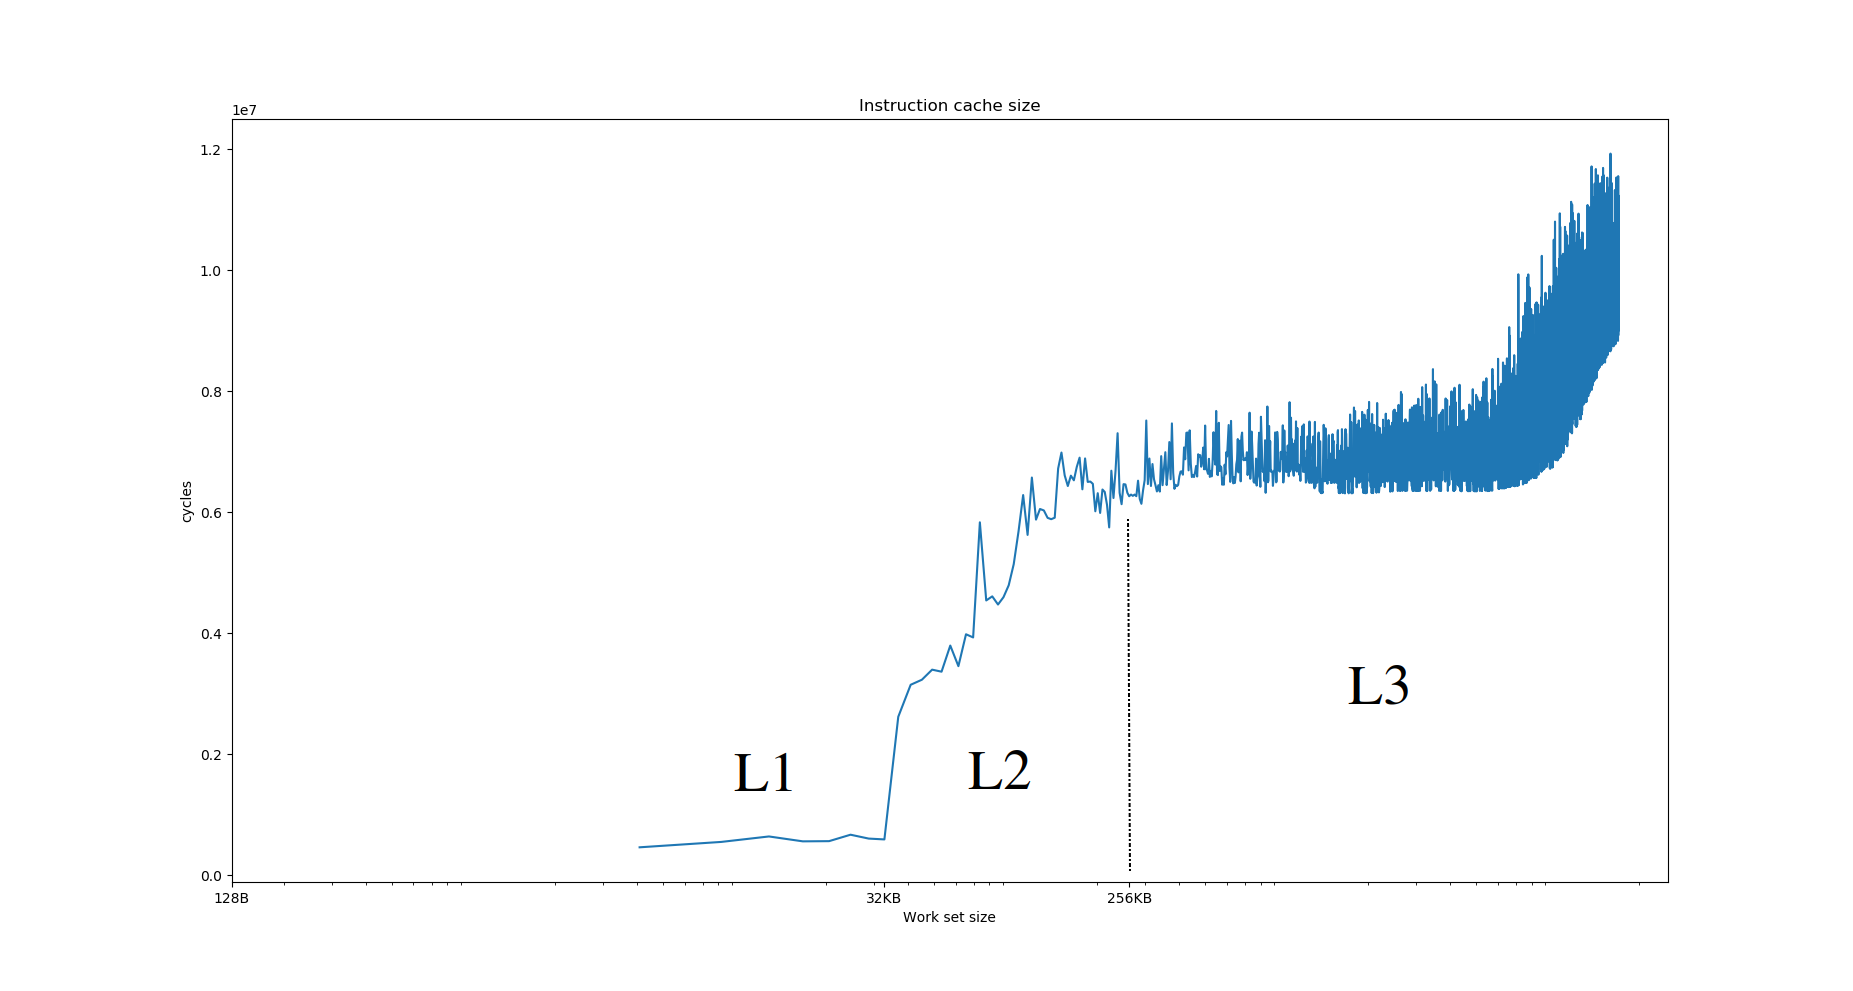
\includegraphics[scale=.25]{img/instr_size.png}
\end{frame}

\begin{frame}
\frametitle{Measuring L1 D-cache associativity}
\begin{itemize}
\item Use P-chasing again
\item Design work set for conflict misses, not capacity misses
\end{itemize}

\begin{block}{64B line, 32 KB L1 D-cache}
32 KB = $2^{15}$ b\\
Let's assume 8-way associativity\\
Sets = $2^{15}$ / ($2^{3}$ * $2^6$) = $2^6$\\
We have: 6 bits line offset, 6 bits set index, 20 bits tag\\
Thus, 0xBAAD\textbf{A}555 and 0xBAAD\textbf{4}555 go to the same set!
\end{block}
\end{frame}

\begin{frame}
\frametitle{Measuring L1 D-cache associativity - observations}
\begin{itemize}
\item Underestimating the assoc still generates addresses to the same set index\\
But since the work set is small, we will have no conflicts
\item Overestimating the assoc generates addresses to different sets\\
Although we have a bigger working set, we will have no conflicts
\item Thus, it's better to measure the change in cost for a bigger working set under same work set\\
\end{itemize}
\begin{block}{example}
C1 = cost(many accesses 16 lines) / cost(many accesses 8 lines) for a 8-way cache\\
C2 = cost(many accesses 8 lines) / cost(many accesses 4lines) for a 8-way cache\\
C2 will be smaller than C1
\end{block}
The code is messy
\end{frame}

\begin{frame}
\frametitle{L1 D-cache associativity plot}
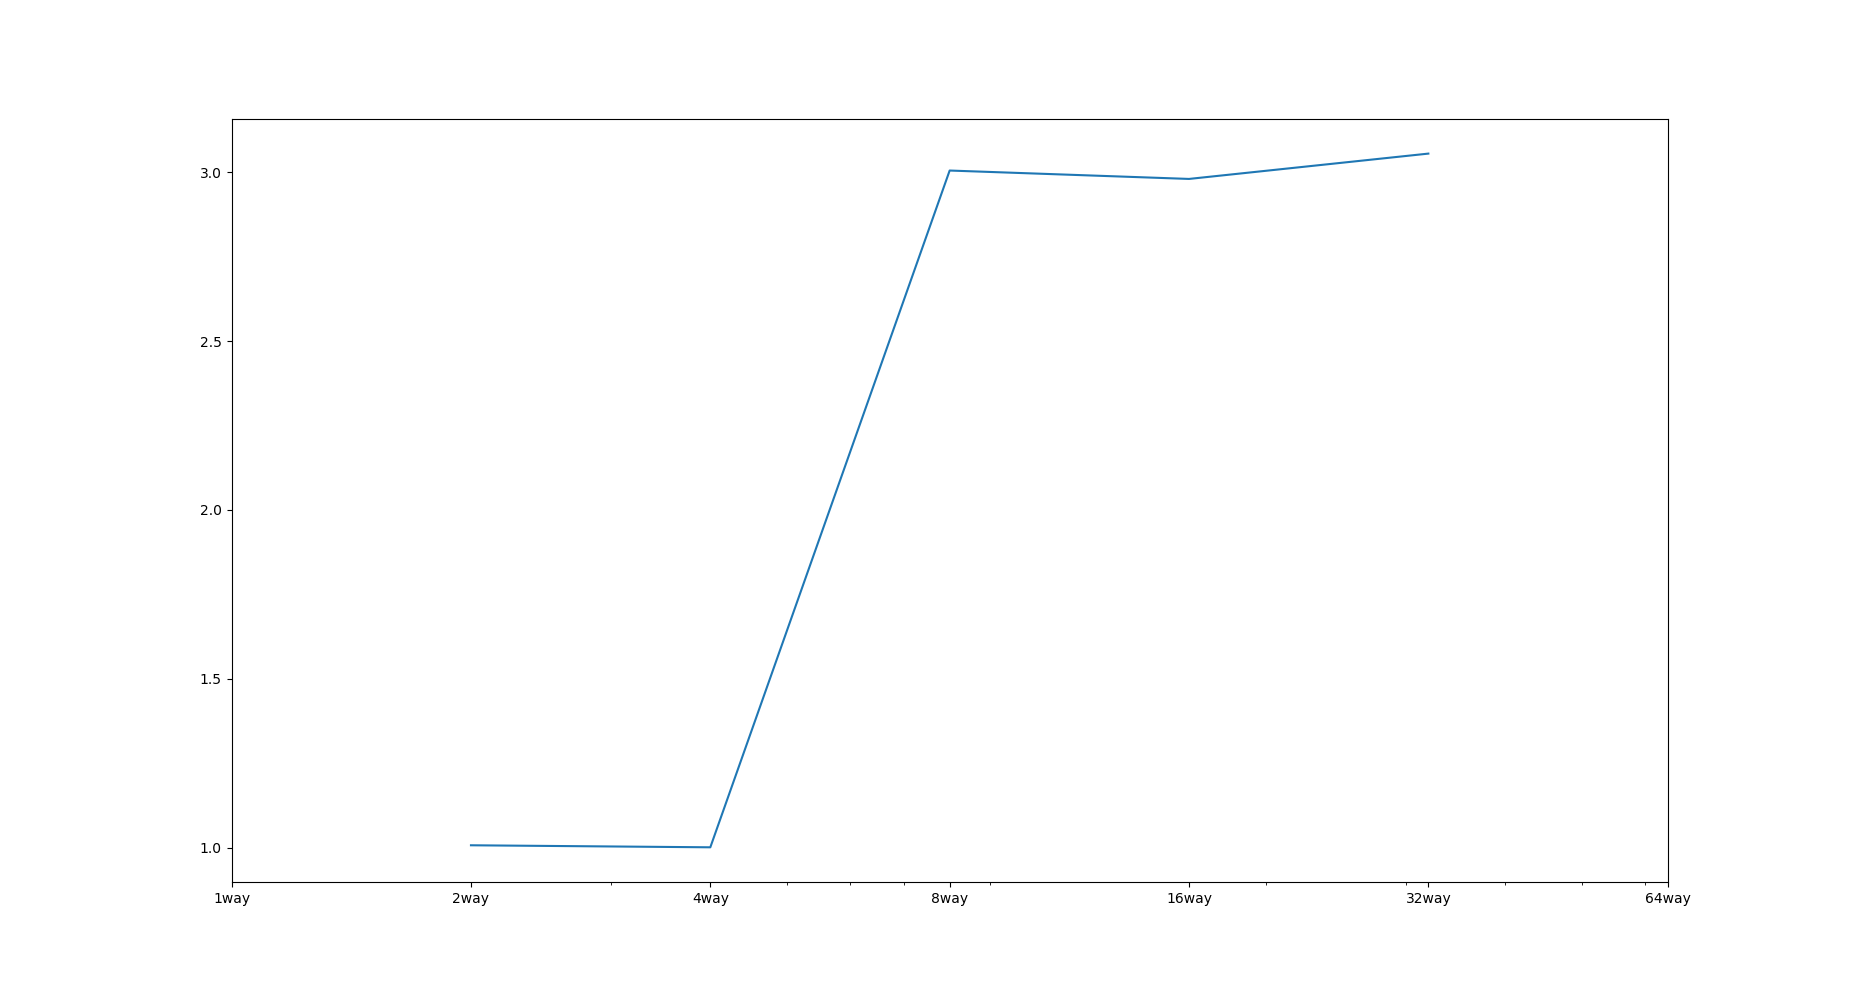
\includegraphics[scale=.25]{img/l1_d_assoc.png}
\end{frame}

\begin{frame}
\frametitle{Timing code on x86}
\begin{itemize}
\item HW register for measuring time - timestamp counter
\item Elapsed cycles since start of core
\item Read through the \textbf{rdtsc} instruction
\item Result stored in \textbf{eax}, \textbf{edx}
\item Can use inline assembly or intrinsics in C/C++/etc.
\end{itemize}
\end{frame}

\begin{frame}[fragile]
\frametitle{RDTSC - issues with reordering}
\begin{block}{Problematic code}
\colorbox{red}{... setup code ... :(} \\
rdtsc\\
... get data from eax, edx into var start ...\\
\colorbox{green}{... run code to benchmark ...}\\
rdtsc\\
... get data from eax, edx into var end ...\\
elapsed = end - start\\
\colorbox{red}{... some other code ... :(}\\
\end{block}
\end{frame}

\begin{frame}[fragile]
\frametitle{RDTSC + CPUID - issues with reordering}
Use CPUID to serialize
\begin{block}{Example code}
\colorbox{green}{... setup code ... :)} \\
cpuid\\
rdtsc\\
... get data from eax, edx into var start ...\\
\colorbox{green}{... run code to benchmark ...}\\
rdtsc\\
... get data from eax, edx into var end ...\\
elapsed = end - start\\
\colorbox{red}{... some other code ... :(}\\
\end{block}
\end{frame}



\begin{frame}
\Huge{\centerline{Thanks for listening}}
\end{frame}

%----------------------------------------------------------------------------------------

\end{document} 
